\chapter{Bush e il Memex, Engelbard e "The Mother of All Demos"}

\section{Introduzione}

\dfn{Knowledge Navigator}{
    Un'idea di Apple, presentata nel 1987, di un assistente virtuale
    che aiuta l'utente a navigare tra le informazioni.
}

\subsubsection{Il filmato di presentazione del Knowledge Navigator (1987):}

\begin{itemize}
    \item [$\Rightarrow$] \fancyglitter{La comprensione del parlato}:
    il computer capisce il linguaggio naturale;
    \item [$\Rightarrow$] \fancyglitter{La grafica e le finestre}:
    dietro questo video c'è Alan Kay, che ha lavorato a Xerox PARC e fu 
    l'inventore delle finestre;
    \item [$\Rightarrow$] \fancyglitter{Il touch screen};
    \item [$\Rightarrow$] \fancyglitter{La videochiamata};
    \item [$\Rightarrow$] \fancyglitter{La simulazione}: della desertificazione.
\end{itemize}

\qs{}{Chi era Vannevar Bush?}

\paragraph{Risposta:} Vannevar Bush (1890 - 1974) era un ingegnere e scienziato americano.
Lui teorizzò il Memex
(non fu mai realizzato).

\nt{Durante una conferenza in occasione del 50° anniversario di "As 
we may think" (1945) venne presentata un'animazione del Memex.}

\section{Il Memex}

\dfn{Memex}{
    Un sistema di archiviazione e ricerca delle informazioni, teorizzato da Vannevar Bush.
}

\nt{Il Memex offre anche un'anticipazione di ciò che sarà l'\fancyglitter{
    ipertesto}, che nascerà vent'anni dopo.
}

\subsection{Problemi di organizzazione dell'informazione}

Il problema che preocupa Bush è \fancyglitter{la perdita di informazioni} che si accumula
continuamente nel tempo\footnote{Questo problema non era nuovo. 
Era già stato affrontato da Paul Otlet.}. Inoltre si aumenta progressivamente la
specializzazione: le informazioni sono sempre più frammentate e sempre più
specializzate (più difficili da comunicare). Bush ritiene che il problema 
non sia l'eccesso di pubblicazioni, ma il fatto che si siano estese oltre
la capacità di gestione dei documenti. 
La \fancyglitter{selezione}\footnote{Processo di scelta delle informazioni.}
è un problema per via delle enormi quantità di informazioni.

\ex{Addetto dell'ufficio informazioni}{
    L’addetto all’ufficio del personale di una fabbrica immette una pila di alcune migliaia di schede
degli impiegati in una macchina selezionatrice, imposta un codice secondo una convenzione
stabilita e produce in poco tempo una lista di tutti gli impiegati che vivono a Trenton e
conoscono lo spagnolo.
}

\ex{Centralini telefonici automatici}{
    Si compone un
numero e la macchina seleziona e connette solamente una tra un milione di possibili stazioni.
Non le ispeziona tutte. Presta attenzione solo a una classe data dalla prima cifra, poi solo a una
sottoclasse data dalla seconda cifra e così via; così procede rapidamente e quasi infallibilmente
verso la stazione selezionata.
}

\paragraph{Prroblemi di indicizzazione:}

\begin{itemize}
    \item [$\Rightarrow$] Si cerca da sottoclasse a sottoclasse;
    \item [$\Rightarrow$] L'informazione si trova in un unico punto (a meno che non sia duplicata);
    \item [$\Rightarrow$] Bisogna avere regole per specificare il percorso, ma le regole sono complicate;
    \item [$\Rightarrow$] Quando si trova l'elemento bisogna riemergere dal sistema e rientrare attraverso un nuovo percorso.
\end{itemize}

\nt{La situazione peggiore, ma più facilmente verificabile, è la ricerca in un albero.}

\dfn{Classificazione}{
    La \newfancyglitter{classificazione} è una segmentazione spaziale, temporale o spazio-temporale del mondo.
    
    Un sistema di classificazione è un insieme di scatole in cui si mettono cose per fare un 
    qualche tipo di lavoro.
}

\paragraph{Proprietà di un sistema di classificazione:}

\begin{itemize}
    \item [$\Rightarrow$] Ci sono principi univoci e consistenti;
    \item [$\Rightarrow$] Le categorie sono reciprocamente esclusive;
    \item [$\Rightarrow$] Il sistema è completo.
\end{itemize}
\pagebreak
\begin{figure}[h]
    \centering
    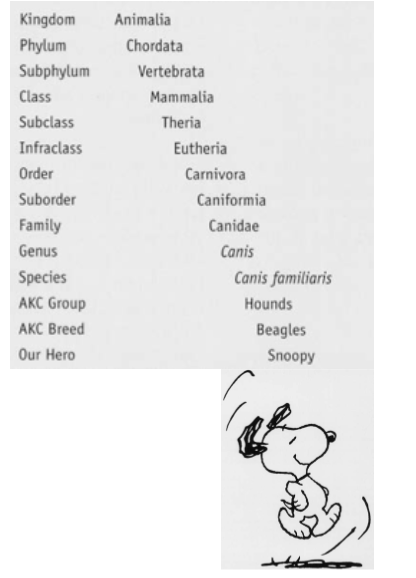
\includegraphics[scale=0.5]{images/Snoopy.png}
    \caption{Snoopy secondo due sistemi di classificazione.}
\end{figure}

\subsection{Indicizzazione}

\dfn{Indicizzazione}{
    L'\newfancyglitter{indicizzazione} è un'operazione è l'azione di descrivere o identificare
    un documento (o un oggetto) nei termini del suo contenuto concettuale\footnote{ISO 5963.}.
}

\nt{Lo scopo generale dell'indicizzazione è quello di rappresentare oggetti
in modo che possano essere efficacemente trovati e utilizzati.}

\cor{Linguaggio di indicizzazione}{
    Un linguaggio di indicizzazione è un sistema di rappresentazioni simboliche (un codice)
    che consentono la classificazione e la ricerca di documenti attraverso
    i codici assegnati ai concetti che essi contengono (indicizzazione per concetti).
}

\nt{Ted Nelson, in "As we may think", criticherà il fraintendimento
per cui si vede nel lavoro di Bush un contributo alla information retrieval\footnote{Reperimento di oggetti informativi.}.
}

\pagebreak

\begin{figure}
    \centering
    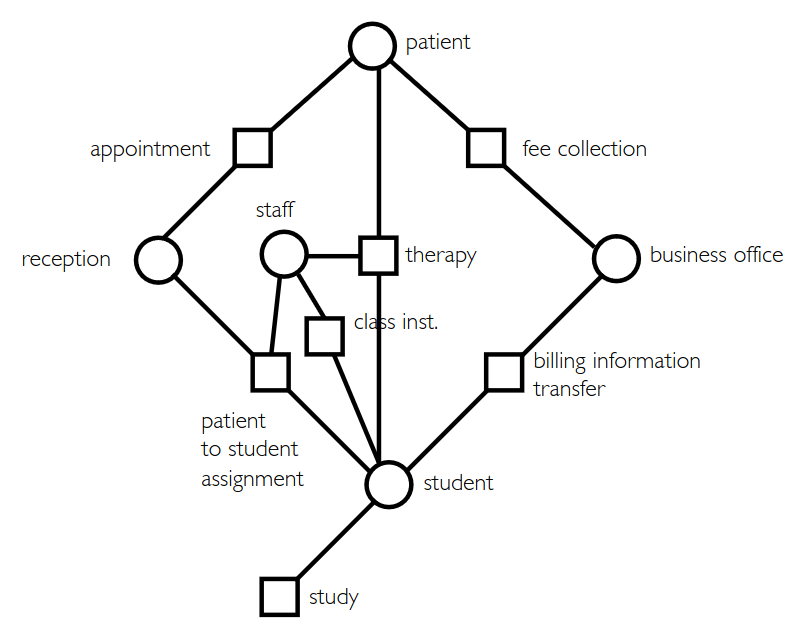
\includegraphics[scale=0.5]{images/UniBoston.png}
    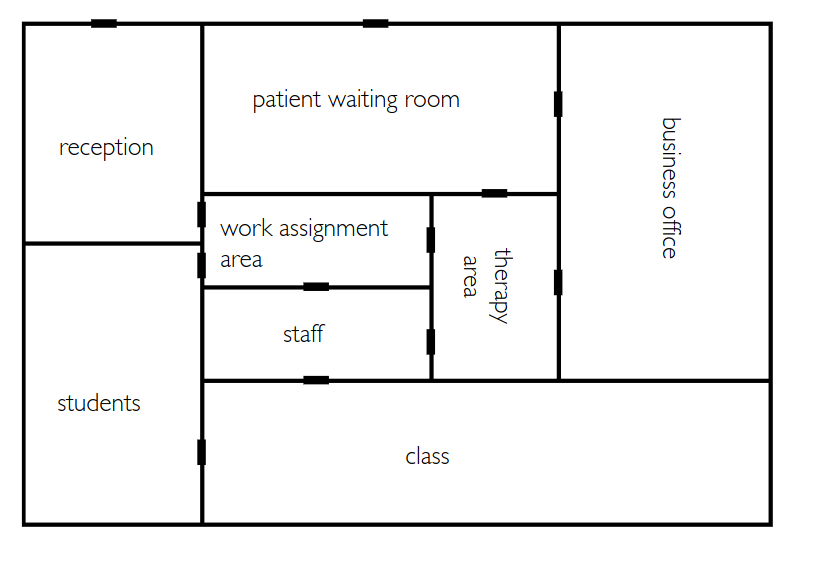
\includegraphics[scale=0.5]{images/UniBoston2.png}
    \caption{Il sistema di classificazione della scuola dentistica dell'Università di Boston.}
\end{figure}




